\chapter{Resultados e discussões}
\label{chap:resultados}

Lorem ipsum dolor sit amet, consectetur adipiscing elit. Vivamus eu magna cursus, mattis velit et, pulvinar lorem. Integer ut nulla eget tellus luctus pellentesque. Nullam fermentum arcu sed tristique congue. Sed ut augue a turpis imperdiet maximus vitae accumsan nisi. Fusce vitae dapibus orci. Pellentesque rutrum tincidunt turpis, id blandit libero lacinia eu. Nunc imperdiet dolor scelerisque ex tristique, nec elementum sem iaculis.


\section{Testes automatizados}\label{tdd}
Esta seção avalia de forma sistemática toda a implementação técnica desenvolvida até o momento, busca uma melhor eficiência e qualidade do código da aplicação. Serão realizados quatro tipos de testes automatizados no Mercado Universitário. Testes unitários e integração, testes de segurança e testes de qualidade do código, tais testes serão apresentados a seguir.
\subsection{Testes unitários e integração}
Foi utilizada a gem RSpec para esse tipo de teste. Tal ferramenta foi apresentada na seção \ref{rspec}. De acordo com a imagem \ref{fig:rspec} foram realizados 102 exemplos de testes na aplicação, tais testes conseguiram cobrir 92.9\% de todo o código da aplicação sem que ocorresse nenhuma falha. Tal resultado se mostra bastante satisfatório, uma vez que se aproxima bastante de 100\% de cobertura do código e não apresenta nenhuma falha.
\begin{figure}[htbp!]
  \centering
  \caption{Saída do terminal para teste automatizado unitário e de integração utilizando a \textit{gem} RSpec}
  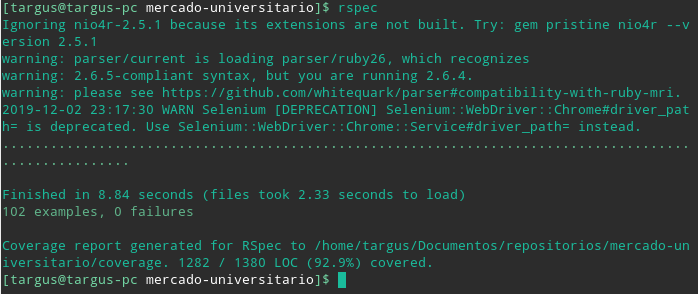
\includegraphics[width=1\textwidth]{figs/rspec.png}
    \legend{Fonte: Elaborada pelo autor.}
    \label{fig:rspec}
\end{figure}
\subsection{Testes de segurança}
Foram utilizadas duas \textit{gems} para realizar esse teste de grande importância para a aplicação. A \textit{gem} Brakeman em conjunto com a \textit{gem} Bundle Audit são suficientes para explorar as principais vulnerabilidades das aplicações web. Como é observado nas imagens \ref{fig:brakeman} e \ref{fig:audit}, não foram encontradas nenhuma vulnerabilidade na aplicação.
\begin{figure}[htbp!]
  \centering
  \caption{Saída do terminal para teste automatizado de segurança utilizando a \textit{gem} Brakeman}
  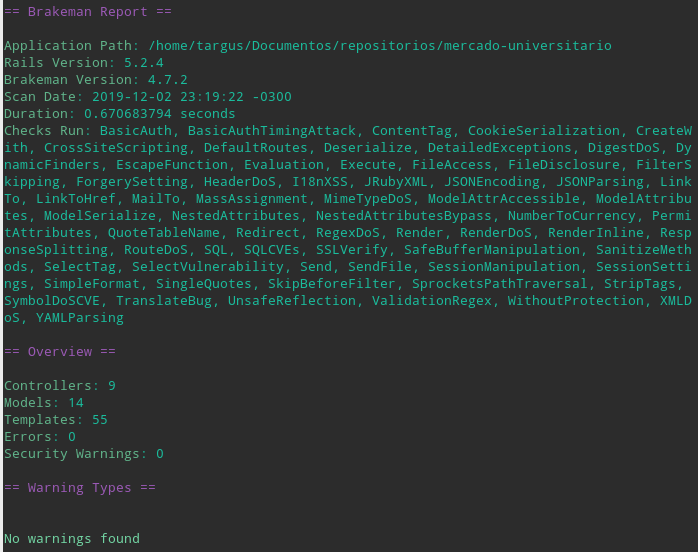
\includegraphics[width=1\textwidth]{figs/brakeman.png}
    \legend{Fonte: Elaborada pelo autor.}
    \label{fig:brakeman}
\end{figure}
\begin{figure}[htbp!]
  \centering
  \caption{Saída do terminal para teste automatizado de segurança utilizando a \textit{gem} Bundle Audit}
  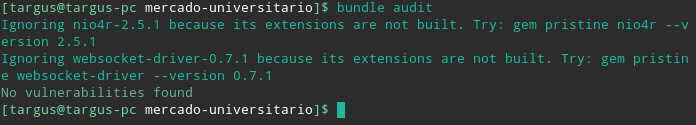
\includegraphics[width=1\textwidth]{figs/bundle_audit.png}
    \legend{Fonte: Elaborada pelo autor.}
    \label{fig:audit}
\end{figure}
\subsection{Testes de qualidade do código}
Para ser possível garantir uma boa manutenção e legibilidade futura do código, foi necessário utilizar a \textit{gem} Rubocop(apresentada na seção \ref{rubocop}). Como observado na imagem \ref{fig:rubocop}, foram verificadas as boas práticas de programação determinadas pelo Rails em 71 arquivos do projeto, não foi encontrada nenhuma ofensa no código.
\begin{figure}[htbp!]
  \centering
  \caption{Saída do terminal para verificação da qualidade do código utilizando a gem Rubocop}
  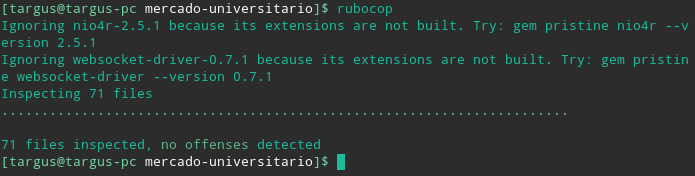
\includegraphics[width=1\textwidth]{figs/rubocop.png}
    \legend{Fonte: Elaborada pelo autor.}
    \label{fig:rubocop}
\end{figure}
